\documentclass[nobib]{tufte-book}

\hypersetup{colorlinks}% uncomment this line if you prefer colored hyperlinks (e.g., for onscreen viewing)

%%
% Book metadata
\title{Notes on String Algorithms}
\subtitle{With Applications in Computational Biology}
\author{Kevin Gao}

%%
% If they're installed, use Bergamo and Chantilly from www.fontsite.com.
% They're clones of Bembo and Gill Sans, respectively.
%\IfFileExists{bergamo.sty}{\usepackage[osf]{bergamo}}{}% Bembo
%\IfFileExists{chantill.sty}{\usepackage{chantill}}{}% Gill Sans
%\usepackage{microtype}

\usepackage[square,numbers]{natbib}

%%
% Just some sample text
\usepackage{lipsum}

%%
% For nicely typeset tabular material
\usepackage{booktabs}

%%
% For graphics / images
\usepackage{graphicx}
\setkeys{Gin}{width=\linewidth,totalheight=\textheight,keepaspectratio}
\graphicspath{{figures/}}

% The fancyvrb package lets us customize the formatting of verbatim
% environments.  We use a slightly smaller font.
\usepackage{fancyvrb}
\fvset{fontsize=\normalsize}

%%
% Prints argument within hanging parentheses (i.e., parentheses that take
% up no horizontal space).  Useful in tabular environments.
\newcommand{\hangp}[1]{\makebox[0pt][r]{(}#1\makebox[0pt][l]{)}}

%%
% Prints an asterisk that takes up no horizontal space.
% Useful in tabular environments.
\newcommand{\hangstar}{\makebox[0pt][l]{*}}

%%
% Prints a trailing space in a smart way.
\usepackage{xspace}

%%
% For typesetting pseudocode
\usepackage{clrscode3e}

%%
% For typesetting math
\usepackage{amsmath}
\usepackage{amssymb}
\usepackage{amsthm}

%%
% For multiple columns typesetting
\usepackage{multicol}

\setcounter{tocdepth}{0}
\setcounter{secnumdepth}{0}
%%
% Theorem environments
\newtheorem{theorem}{Theorem}[chapter]
\newtheorem{lemma}[theorem]{Lemma}
\newtheorem{claim}[theorem]{Claim}
\newtheorem{corollary}[theorem]{Corollary}
\newtheorem{definition}[theorem]{Definition}
\newtheorem{rules}[theorem]{Rule}
\newtheorem{remark}[theorem]{Remark}
\newtheorem{example}[theorem]{Example}

% Prints the month name (e.g., January) and the year (e.g., 2008)
\newcommand{\monthyear}{%
  \ifcase\month\or January\or February\or March\or April\or May\or June\or
  July\or August\or September\or October\or November\or
  December\fi\space\number\year
}


% Prints an epigraph and speaker in sans serif, all-caps type.
\newcommand{\openepigraph}[2]{%
  %\sffamily\fontsize{14}{16}\selectfont
  \begin{fullwidth}
  \sffamily\large
  \begin{doublespace}
  \noindent\allcaps{#1}\\% epigraph
  \noindent\allcaps{#2}% author
  \end{doublespace}
  \end{fullwidth}
}

% Inserts a blank page
\newcommand{\blankpage}{\newpage\hbox{}\thispagestyle{empty}\newpage}

\usepackage{units}

% Typesets the font size, leading, and measure in the form of 10/12x26 pc.
\newcommand{\measure}[3]{#1/#2$\times$\unit[#3]{pc}}

% Macros for typesetting the documentation
\newcommand{\hlred}[1]{\textcolor{Maroon}{#1}}% prints in red
\newcommand{\hangleft}[1]{\makebox[0pt][r]{#1}}
\newcommand{\hairsp}{\hspace{1pt}}% hair space
\newcommand{\hquad}{\hskip0.5em\relax}% half quad space
\newcommand{\TODO}{\textcolor{red}{\bf TODO!}\xspace}
\newcommand{\na}{\quad--}% used in tables for N/A cells
\providecommand{\XeLaTeX}{X\lower.5ex\hbox{\kern-0.15em\reflectbox{E}}\kern-0.1em\LaTeX}
\newcommand{\tXeLaTeX}{\XeLaTeX\index{XeLaTeX@\protect\XeLaTeX}}
% \index{\texttt{\textbackslash xyz}@\hangleft{\texttt{\textbackslash}}\texttt{xyz}}
\newcommand{\tuftebs}{\symbol{'134}}% a backslash in tt type in OT1/T1
\newcommand{\doccmdnoindex}[2][]{\texttt{\tuftebs#2}}% command name -- adds backslash automatically (and doesn't add cmd to the index)
\newcommand{\doccmddef}[2][]{%
  \hlred{\texttt{\tuftebs#2}}\label{cmd:#2}%
  \ifthenelse{\isempty{#1}}%
    {% add the command to the index
      \index{#2 command@\protect\hangleft{\texttt{\tuftebs}}\texttt{#2}}% command name
    }%
    {% add the command and package to the index
      \index{#2 command@\protect\hangleft{\texttt{\tuftebs}}\texttt{#2} (\texttt{#1} package)}% command name
      \index{#1 package@\texttt{#1} package}\index{packages!#1@\texttt{#1}}% package name
    }%
}% command name -- adds backslash automatically
\newcommand{\doccmd}[2][]{%
  \texttt{\tuftebs#2}%
  \ifthenelse{\isempty{#1}}%
    {% add the command to the index
      \index{#2 command@\protect\hangleft{\texttt{\tuftebs}}\texttt{#2}}% command name
    }%
    {% add the command and package to the index
      \index{#2 command@\protect\hangleft{\texttt{\tuftebs}}\texttt{#2} (\texttt{#1} package)}% command name
      \index{#1 package@\texttt{#1} package}\index{packages!#1@\texttt{#1}}% package name
    }%
}% command name -- adds backslash automatically
\newcommand{\docopt}[1]{\ensuremath{\langle}\textrm{\textit{#1}}\ensuremath{\rangle}}% optional command argument
\newcommand{\docarg}[1]{\textrm{\textit{#1}}}% (required) command argument
\newenvironment{docspec}{\begin{quotation}\ttfamily\parskip0pt\parindent0pt\ignorespaces}{\end{quotation}}% command specification environment
\newcommand{\docenv}[1]{\texttt{#1}\index{#1 environment@\texttt{#1} environment}\index{environments!#1@\texttt{#1}}}% environment name
\newcommand{\docenvdef}[1]{\hlred{\texttt{#1}}\label{env:#1}\index{#1 environment@\texttt{#1} environment}\index{environments!#1@\texttt{#1}}}% environment name
\newcommand{\docpkg}[1]{\texttt{#1}\index{#1 package@\texttt{#1} package}\index{packages!#1@\texttt{#1}}}% package name
\newcommand{\doccls}[1]{\texttt{#1}}% document class name
\newcommand{\docclsopt}[1]{\texttt{#1}\index{#1 class option@\texttt{#1} class option}\index{class options!#1@\texttt{#1}}}% document class option name
\newcommand{\docclsoptdef}[1]{\hlred{\texttt{#1}}\label{clsopt:#1}\index{#1 class option@\texttt{#1} class option}\index{class options!#1@\texttt{#1}}}% document class option name defined
\newcommand{\docmsg}[2]{\bigskip\begin{fullwidth}\noindent\ttfamily#1\end{fullwidth}\medskip\par\noindent#2}
\newcommand{\docfilehook}[2]{\texttt{#1}\index{file hooks!#2}\index{#1@\texttt{#1}}}
\newcommand{\doccounter}[1]{\texttt{#1}\index{#1 counter@\texttt{#1} counter}}

\newcommand{\N}{\mathbb{N}}
\newcommand{\Z}{\mathbb{Z}}
\newcommand{\R}{\mathbb{R}}
\newcommand{\Q}{\mathbb{Q}}

% Generates the index
\usepackage{makeidx}
\makeindex


\titlecontents{part}
    [0pt]
    {\addvspace{0.25\baselineskip}}
    {{Part~\thecontentslabel}}
    {{Part~\thecontentslabel}}
    {}
    [\vspace*{0.5\baselineskip}]

\titlecontents{chapter}
    [4em]
    {}
    {\contentslabel{2em}\textit}
    {\hspace{0em}\textit}
    {\qquad\thecontentspage}
    [\vspace*{0.5\baselineskip}]

\begin{document}

% Front matter
\frontmatter

% r.1 blank page

% v.2 epigraphs

% r.3 full title page
\maketitle


% v.4 copyright page
\newpage
\begin{fullwidth}
~\vfill
\thispagestyle{empty}
\setlength{\parindent}{0pt}
\setlength{\parskip}{\baselineskip}
Copyright \copyright\ \the\year\ \thanklessauthor

\par\smallcaps{terra-incognita.dev}

\par Licensed under the Apache License, Version 2.0 (the ``License''); you may not
use this file except in compliance with the License. You may obtain a copy
of the License at \url{http://www.apache.org/licenses/LICENSE-2.0}. Unless
required by applicable law or agreed to in writing, software distributed
under the License is distributed on an \smallcaps{``AS IS'' BASIS, WITHOUT
WARRANTIES OR CONDITIONS OF ANY KIND}, either express or implied. See the
License for the specific language governing permissions and limitations
under the License.


\end{fullwidth}

% r.5 contents
\tableofcontents

% r.7 dedication
\cleardoublepage
~\vfill

{\noindent\fontsize{18}{22}\selectfont\itshape
These notes are primarily based on the book \textbf{Algorithms on Strings, Trees, and Sequences} by \textbf{Dan Gusfield} \cite{gusfield_1997}.

\hfill

\noindent Thanks Professor Gusfield for his great book.

\hfill

The part on indexing and compression is based on the book \textbf{Genome-Scale Algorithm Design} \cite{makinen_belazzougui_cunial_tomescu_2015} and Ben Langmead's lectures.
}

\vfill
\vfill


% r.9 introduction
\cleardoublepage

% \chapter*{Notations}

% \section*{Strings}

% Strings are denoted by $S$. When we need to distinguish the text from the pattern, we use $T$ and $P$, respectively.

% Prefix of a string ending at index $i$ is denoted by $S[\ldots i]$. Similarly, suffix of a string starting at index $i$ is denoted by $S[i \ldots]$. Indicies start at $1$.

% \section*{Sets}

% Natural number: $\N$

% Postive natural numbers: $\N^+$, $0 \not\in \N^+$

% Integers: $\Z$

% Postivie natural numbers from $1$ to $n$: $[n] = \{ i \in \N^+ \mid i \leq n \}$

% Reals: $\R$

%%
% Start the main matter (normal chapters)
\mainmatter

\part{Comparison-Based Exact Matching}

\chapter{Naive Exact Matching}
(Gusfield Section 1.1)

\newthought{Terminology Confusion}. Before starting the discussion of string matching algorithms, we should note the difference between a \textit{\textbf{substring}} and a \textit{\textbf{subsequence}}. Given a string S, characters in a substring of S must occur contiguously in S; whereas characters in a subse- quence may be interspersed gaps (or indels, as we call them in biology) and/or characters not in the original string.

\section{Exact String Mathching Problem}

Given a text string $T$ and pattern $P$, the goal of the exact string matching problem is to find all occurrences of $P$ in $T$.

\section{The ``Na\"ive'' Algorithm} \index{naive exact matching algorithm}

\begin{codebox}
    \Procname{$\proc{Naive-Match}(P,T)$}
    \li $\id{matches} = [\;]$
    \li \For $i=1$ \To $|T|-|P|+1$ \Do
        \li $\id{match} = \const{true}$
        \li \For $j = 1$ \To $|P|$ \Do
            \li \If $T[i+j] \neq P[j]$ \Then
                \li $\id{match} = \const{false}$
                \li \textbf{break}
            \End
        \li \If $\id{match}$ \Then
            \li $\id{matches}.\proc{Append}(i)$ 
        \End
    \End
    \li \Return $\id{matches}$ 
\end{codebox}

\begin{marginfigure}
    \caption{Naive exact matching with $P=abxyabxa$ and $T=xabxyabxyabxz$.}
    \begin{alignat*}{7}
        T:\; &x&&a&&b&&x&&y&&abxyabxz \\
        P:\; &a&&b&&x&&y&&a&&bxa \\
        & && a&&b&&x&&y&&abxa \\
        & && && a&&b&&x&&yabxa \\
        & && && && a&&b&&xyabxa \\
        & && && && && a &&bxyabxa \\
        & && && && && && abxyabxa \\
    \end{alignat*}
    \label{fig:naive-matching}
\end{marginfigure}

The na\"ive exact matching algorithm aligns the left end of $P$ with the left end of $T$ and compares the characters of $P$ and $T$ left to right until a mismatch is found, or until it reaches the end of $P$, in which case we report the position of $P$. Then, $P$ is shifted to the right by one place. We repeat this procedure until the right end of $P$ passes the right end of $T$.

\section{Runtime of the Naive Algorithm}

Let $n = |P|$ and $m = |T|$. The worst-case comparisons made by the naive algorithm is $\Theta(nm)$. We have the lower bound $\Omega(nm)$ when
$P$ and $T$ contains the same repeated characters (e.g. $P = aaa$, $T = aaaaaaaaa$), in which case the algorithm makes $n(m-n+1) \in \Omega(nm)$ comparisons.

\chapter{Z Algorithm}
(Gusfield Chapter 1)

\section{Speeding Up the Naive Algorithm}

The naive exact matching algorithm is stupid. It always shifts $P$ by only one even if it knows for sure that the next shift will not yield a match. This gives us some ideas on how to improve the algorithm. If we can shift $P$ by more than one character, but never shift so far as to miss the next occurrence of $P$ in $T$, we can improve the runtime of the naive algorithm.

Doing this, however, requires us to have some prior knowledge of the pattern $P$ or the text $T$.

\section{Foundamental Preprocessing}

A fundemental preprocessing is a generalized way to process the pattern $P$ to gain knowledge of the pattern, independent of any particular algorithm.

\begin{definition}
    Given a string $S$ and a position $i>1$, let $Z_i(S)$ be the length of the longest substring of $S$ that starts at $i$ and matches a prefix of $S$.

    In other words, $Z_i(S)$ is the length of the longest prefix of $S[i\ldots |S|]$ that matches a prefix of $S$.
\end{definition}

\begin{definition}[Z-box] \index{Z-box}
    For any position $i > 1$ where $Z_i$ is greater than 0, the \textbf{Z-box} at $i$ is the interval starting at $i$ and ending at $i+Z_i-1$.
\end{definition}

\begin{marginfigure}
    \includegraphics[width=\linewidth]{z/z-box.pdf}
    \caption{Relations between $i$, $l_i$, $r_i$ and the Z-box at $l_i$.}
    \label{fig:z-box}
\end{marginfigure}

\begin{definition}
    For every $i > 1$, $r_i$ is the right endpoint of the Z-box that begins at or befor position $i$ (i.e. the closest Z-box to the left). More formally, $r_i$ is the largest value of $j + Z_j - 1$ over all $1 < j \leq i$ such that $Z_j > 0$.
\end{definition}

\index{fundamental preprocessing}
The linear-time computation of the $Z_i$ values for all $i \in \{1,\ldots,|S|\}$ from the string $S$ is called the \textit{\textbf{fundamental preprocessing}} task.

\section{The Z Algorithm} \index{Z algorithm}

The \textit{\textbf{Z algorithm}} is an algorithm for computing the fundamental preprocessing. The Z algorithm is similar to a dynamic programming algorithm in the sense that it uses memoized information to speed up the computation and reduce the number of comparison needed. Namely, assume there exists $j < i$ such that $j + Z[j] - 1 > i$, then we can use $Z[i-j+1]$ to infer $Z[i]$.

\begin{figure}[htbp]
    \centering
    \includegraphics[width=\linewidth]{z/z-process-case2a.pdf}
    \caption{Case 2a: The longest string starting at $k'$ that matches a prefix of $S$ is shorter than $|\beta| = r-k+1$. In this case, $Z_k = Z_{k'}$.}
    \label{fig:z-process-case2a}
\end{figure}

\begin{figure}[htbp]
    \centering
    \includegraphics[width=\linewidth]{z/z-process-case2b1.pdf}
    \includegraphics[width=\linewidth]{z/z-process-case2b2.pdf}
    \caption{Case 2b: The longest string starting at $k'$ that matches a prefix of $S$ is at least $|\beta| = r-k+1$. In this case, we continue to compare characters right of $r$ with characters right of the $Z_{k'}$th character until mismatch. }
    \label{fig:z-process-case2b}
\end{figure}

Given $Z_i$ for all $1 < i \leq k-1$ and the current $l$ and $r$, we can compute $Z_k$ using the following procedure:

\begin{enumerate}
    \item Case 1: If $k > r$, $k$ is not in an existing Z-box. Compute $Z_k$ by explicitly comparing each character starting at $k$ with prefix of $S$.
    \item Case 2: If $k \leq r$, $k$ is in an existing Z-box, denoted $\alpha$, that matches a prefix of $S$. Hence, character $S[k]$ also appears in the prefix at position $k' = k - l + 1$. \\ We also consider the substring $S[k\ldots r]$, denoted $\beta$. By the same reasoning, $\beta$ matches the substring $S[k'\ldots Z_l]$.
    \begin{enumerate}
        \item $Z_{k'} < |\beta|$. This implies that the longest string starting at $k'$ that matches a prefix of $S$, $\gamma$, is shorter $|\beta|$. Then, $Z_{k} = Z_{k'}$, and $l,r$ remain unchanged. Note that $|\gamma|$ can be 0.
        \item $Z_{k'} \geq |\beta|$. This means $S[k\ldots r]$ is at least a prefix of $S$. However, $Z_k$ might be larger than $|\beta|$. We cannot determine this solely based on the existing information as characters beyond the $Z_l$th character are not included in $\alpha$. So, we compare the characters starting at position $r+1$ of $S$ to the characters starting at position $|\beta|+1$ of $S$, until a mismatch occurs. Say the mismatch occur at position $q$. Then, $Z_k = q- k$, $r = q-1$, and $l = k$. (If $Z_{k'} > |\beta|$, a mismatch occurs immediate after the $Z_{l}$th character because otherwise, the $(r+1)$th character matches the $Z_{l}$th character, and we would have a longer $\alpha$ and a larger $Z_l$)
    \end{enumerate}
\end{enumerate}

\begin{codebox}
    \Procname{$\proc{Compute-Z}(S)$}
    \li $n = |S|$
    \li $l,r,k = 1$
    \li $Z = \text{empty array of length $n$}$
    \li \For $k=2$ \To $n$ \Do
        \li \If $k > r$ \Then \RComment{Case 1}
            \li \Comment{compute $Z[k]$ from scratch}
            \li $l,r = k$ 
            \li \While $r \leq n$ \textbf{and} $S[r-l+1] \isequal S[r]$ \Do
                \li $r = r + 1$
            \End
            \li $Z[k] = r-l$
            \li $r = r - 1$
        \li \Else \RComment{Case 2}
            \li $k' = k - l + 1$
            \li \If $Z[k'] < r - k + 1$ \Then \RComment{Case 2a}
                \li $Z[k] = Z[k']$ 
            \li \Else \RComment{Case 2b}
                \li $q = r+1$
                \li \While $q \leq n$ \textbf{and} $S[q-l + 1] \isequal S[q]$ \Do
                    \li $q = q + 1$
                \End
                \li $Z[k] = q-k$
                \li $l,r = k, \,q-1$ 
            \End
        \End
        \End
        \li \Return $Z$ 
\end{codebox}

For a step-by-step animation of the Z algorithm, see \\
\href{https://personal.utdallas.edu/~besp/demo/John2010/z-algorithm.htm}{https://personal.utdallas.edu/\textasciitilde besp/demo/John2010/z-algorithm.htm}

\section{Running Time of the Z Algorithm}

\begin{theorem}
    All the $Z_i$ values can be computed by the Z algorithm with at most $2|S| \in O(|S|)$ comparisons.
\end{theorem}

\begin{proof}
    The time is proportional to the number of iterations, $|S|$, plus the number of character comparisons.
    
    Each iteration that does any character comparison ends as soon as there is a mismatch, so there are at most $|S|$ \textbf{mismatches}. In every iteration where there is a match, $r$ moves to the right by an amount at least as large as the number of matches. This implies that there are at most $|S|$ \textbf{matches}. Note that once a character results in a match, it is not compared again.

    Every character comparison is either a match or mismatch, so the total number of comparisons is at most $2|S|$.
\end{proof}

\section{Correctness of the Z Algorithm}

\begin{theorem}
    At the $k$th iteration of the algorithm, \proc{Compute-Z} correctly calculates $Z_k$, and $l,r$ are updated correctly.
\end{theorem}

\begin{proof}
    By a case analysis.

    Case 1: Trivial since it's just explicit comparison.

    Case 2a: We claim that the substring at position $k$ can match a prefix of $S$ only for length $Z_{k'} < |\beta|$. Prove the claim by contradiction (suppose not, we would have a longer prefix matching the substring at $k'$, contradicting the maximality of $Z_{k'}$).

    Case 2b: $\beta$ must be a prefix of $S$ as established above. Characters beyond $r$ are explicitly compared.
\end{proof}

\begin{corollary}
    \proc{Compute-Z} correctly calculates $Z_k$ for all $k \in \{2,\ldots,|S|\}$.
\end{corollary}

\begin{proof}
    By induction on $k$.
\end{proof}

\section{Z Algorithm for Exact Matching}

The Z algorithm lends itself to a linear-time algorithm for exact matching. Given a pattern $P$ and text $T$, we construct a new string $P \$ T$ where $\$$ is a \textit{\textbf{separator}} (a.k.a. \textit{\textbf{delimiter}} or \textit{\textbf{sentinel}}) such that $\$ \not\in \Sigma$. We construct the Z-array for this new string. It takes $O(|P|+|T|)$ time to construct the Z-array. After this, we can simply make a pass through the Z-array and read the result from it. This takes $O(|T|)$ time.

\begin{codebox}
    \Procname{$\proc{Z-Exact-Matching}(P,T)$}
    \li $\id{query} = P + ``\$" + T$
    \li $Z = \proc{Compute-Z}(\id{query})$
    \li \For $i = |P|+1$ \To $|P|+|T|+1$ \Do
        \li \If $Z[i] \isequal |P|$ \Then
            \li pattern found at index $i - |P|$ 
\end{codebox}

\chapter{Boyer-Moore}
(Gusfield Chapter 2)

\newthought{Key Ideas} of the Boyer-Moore algorithm: right-to-left scan, bad character rule, good suffix rule.

\section{Bad Character Rule}

The intuition behind the bad character rule is as follows. Suppose we have the pattern $P$ and text $T$, and the rightmost character of $P$ is aligned to the character $x$ in $T$, where $x \neq y$. If we know the position of the rightmost $x$ in $P$, we can safely shift $P$ by that amount to the right so that the $x$ in $P$ aligns with the $x$ in $T$. Furthermore, if we know that $x$ is not in $P$, we can shift $P$ completely past the $x$ in $T$. This intuition is formalized below, as shown in Gusfield's book.

\begin{definition}
    For each character $x$ in the alphabet, let $R(x)$ be the position of the rightmost occurrence of character $x$ in $P$. If $x$ does not occur in $P$, $R(x) = 0$.
\end{definition}

\begin{rules}[Bad Character Rule] \index{bad character rule}
    \normalfont
    Suppose for a particular alignment of $P$ against $T$, the rightmost $n-i$ characters of $P$ match their counterparts in $T$, but the next character to the left $P(i)$ mismatches with its counterpart in $T$, say at position $k$ in $T$. The \textit{\textbf{bad character rule}} says that $P$ should be shifted right by $\max\{1,\, i-R(T(k))\}$ places. That is, if the rightmost occurrence of $T(k)$ in $P$ is in position $j < i$, then shift $P$ so that the $j$th character of $P$ is matched to the $k$th character of $T$ (or completely shifting $P$ past $k$th position if the $k$th character of $T$ does not occurr in $P$). Otherwise, if $j > i$, shift $P$ by one position.
\end{rules}

\section{Extended Bad Character Rule}

Note that the bad character rule allows us to shift more than one character only when the mismatched character show up at a position left of the mismatched point. However, it is not as helpful if the character only occurs in $P$ on the right side of the mismatched point. The \textit{\textbf{extended bad character rule}} addresses this issue.

\begin{rules}[Extended Bad Character Rule] \index{extended bad character rule}
    \normalfont
    When a mismatch occurs at position $i$ of $P$ and the mismatched character in $T$ is $x$, then shift $P$ to the right so that the closest $x$ to the left position $i$ in $P$ is matched with the $x$ in $T$.
\end{rules}

\begin{figure}[htbp]
    \centering
    \includegraphics[width=0.8\linewidth]{boyer-moore/bad-character-rule.pdf}
    \caption{The bad character rule says to shift as much as possible so that a mismatch becomes a match.}
    \label{fig:boyer-moore-bad-char-rule}
\end{figure}

\subsection{Preprocessing for Bad Character Rule}

The bad character rule is quite straightforward to implement. In the preprocessing for the bad character rule, we find, for each position $i$ in the pattern $P$ and for each characther $x \in \Sigma$, the position of the closest occurrence of $x$ in $P$ to the left of $i$. This uses an $n \time \Sigma$ matrix. However, the time complexity for building this lookup table and the space required for it could be massive, depending on the length of the pattern and the size of the alphabet. It is also not hard to see that this approach can be quite space inefficient and we can end up store duplicate information over and over.

\begin{marginfigure}
    \includegraphics[width=0.5\linewidth]{boyer-moore/bad-character-rule-table.pdf}

    \hfill
    
    \caption{Table for storing information obtained from the bad character rule preprocessing.}
    \label{fig:bad-character-rule-table}
\end{marginfigure}

Alternatively, we can scan $P$ from right to left, and for each character $x \in \Sigma$, we keep a list of positions where $x$ occurs in $P$ (think hash table with chaining but just using another array instead of linked list). Since we scan $P$ from right to left, the indices will be stored in decreasing order for each character. It takes $O(n)$ space. During the actual execution of the Boyer-Moore algorithm, we can query this table whenever we need to find the rightmost occurrence of character $x$ left of index $i$. We can use \textit{binary search} for this.

If the alphabet $\Sigma$ is sparse, we can condense it by simply creating a mapping $f$ from $\Sigma \to \N$. The two approaches can be implemented as follows, respectively.

\begin{multicols}{2}
    \begin{codebox}
        \Procname{$\proc{Create-Bad-Char-Table}(P, f)$}
        \li $\id{table} = [\,]$
        \li $\id{row} = [0,\ldots,0]$
        \li \For $i = 1$ \To $|P|$ \Do
            \li $c = P[i]$
            \li $\id{table}.\proc{Append}(\id{row})$
            \li $\id{row}[f(c)] = i + 1$
        \End
        \li \Return $\id{table}$ 
    \end{codebox}
    
    \begin{codebox}
        \Procname{$\proc{Create-Bad-Char-Table}(P, f)$}
        \li $\id{table} = [\,]$
        \li \For $i = |P|$ \textbf{downto} $1$ \Do
            \li $c = P[i]$
            \li $\id{table}[f(c)].\proc{Append}(i)$
        \End
        \li \Return $\id{table}$ 
    \end{codebox}
    
\end{multicols}


\section{Good Suffix Rule}

\begin{rules}[Good Suffix Rule] \index{good suffix rule}
    \normalfont
    Given an alignment of $P$ against $T$, suppose a substring $t$ of $T$ matches a \textbf{suffix} of $P$, but a mismatch occurs at the next comparison to the left. Then, find, if exsits, the right-most copy $t'$ of $t$ in $P$ such that $t'$ is not a suffix of $P$. Shift $P$ to the right so that $t'$ in $P$ is matched with $t$ in $T$.
\end{rules}

Essentially, the \textit{\textbf{good suffix rule}} says we can shift as much as possible such that an \textit{existing match does not become a mismatch}. 

This rule is the weaker version of the good suffix rule used by Boyer and Moore's original publication. We now present a stronger version of the good suffix rule that allows us to prove properties of the Boyer-Moore algorithm more easily.

\section{Strong Good Suffix Rule}

\begin{rules}[Strong Good Suffix Rule] \index{strong good suffix rule}
    \normalfont
    Given an alignment of $P$ against $T$, suppose a substring $t$ of $T$ matches a \textbf{suffix} of $P$, but a mismatch occurs at the next comparison to the left. Then, find, if exsits, the right-most copy $t'$ of $t$ in $P$ such that $t'$ is not a suffix of $P$. Additionally, \textbf{we requires that the character left of $t'$ in $P$ differs from the character to the left of $t$ in $P$}. Shift $P$ to the right so that $t'$ in $P$ is matched with $t$ in $T$.
\end{rules}

\begin{figure}[htbp]
    \centering
    \includegraphics[width=0.6\linewidth]{boyer-moore/good-suffix-rule.pdf}
    \caption{The good suffix rule says we can shift as much as possible so long as a match does not become a mismatch. The additional requirement in the strong good suffix rule ensures that we don't encounter the same mismatch at $P[i-1]$.}
    \label{fig:boyer-moore-good-suffix-rule}
\end{figure}

Note the additional requirement stated in the second-to-last sentence. The addition of this requirement ensures that we don't get the same mismatch. A copy of $t$ is not worth looking at if it results in the same mismatch at the next character to the left. We call this rule the \textit{\textbf{strong good suffix rule}}. It should be obvious that it is safe to shift using the strong good suffix rule. That is, we won't miss any matches if we shift $P$ using the strong good suffix rule. We formalize this idea of correctness in the following theorem.

\begin{theorem}
    The strong good suffix rule does not shift $P$ past an occurrence in $T$.
\end{theorem}

\begin{proof}
    By contradiction. See Gusfield Theorem 2.2.1.
\end{proof}

\subsection{Preprocessing for Good Suffix Rule}


\begin{definition}
    For each $i$, let $L(i)$ be the \textbf{largest position} less than $n$ such that string $P[i\ldots n]$ matches a suffix of $P[1\ldots L(i)]$. If no such position exists, $L(i) = 0$.
    \begin{marginfigure}
        \includegraphics[width=\linewidth]{boyer-moore/good-suffix-Li.pdf}
        \caption{$L(i)$ gives the right-most copy of $t$ that is not a suffix of the whole string.}
        \label{fig:good-suffix-Li}
    \end{marginfigure}
    For each $i$, let $L'(i)$ be the largest position less than $n$ such that string $P[i \ldots n]$ matches a suffix of $P[1\ldots L'(i)]$ and such that the character preceding that suffix is not equal to $P[i-1]$. If no such position exists, $L'(i) = 0$.
\end{definition}

By definition, $L'(i)$ gives the right endpoint of the rightmost copy of $P[i\ldots n]$ that is not a suffix of $P$, and whose preceding character does not equal to $P[i-1]$.

\begin{definition}
    For string $P$, $N_j(P)$ is the length of the \textit{\textbf{longest suffix}} of the substring $P[1\ldots j]$ that is also a \textit{\textbf{suffix}} of the whole string $P$.
\end{definition}

\begin{theorem} \label{thm:good-suffix-Li-property}
    $L(i)$ is the largest index $j$ less than $n$ such that $N_j(P) \geq |P[i\ldots n]|$.
\end{theorem}

\begin{proof}
    By definition of $L$, $L(i)$ is the largest index less than $n$ such that $P[i\ldots n]$ matches a suffix of $P[1\ldots L(i)]$. 
    
    Let $j = L(i)$ in the definition of $N_j$. Then, $N_j(P)$ is the length of the longest suffix of the substring $P[1\ldots L(i)]$ that is also a suffix of the whole string. A suffix of the whole string must also be a suffix of $P[i\ldots n]$. Then, clearly, $N_j(P) \geq |P[i \ldots n]|$ because the substring $P[L(i)-N_j(P)+1 \ldots L(i)]$ can possibly match more characters left of $P[i]$.
\end{proof}

\begin{corollary}
    $L'(i)$ is the largest index $j$ less than $n$ such that $N_i(P) = |P[i\ldots n]| = n-i+1$.
\end{corollary}

\begin{proof}
    Immediate from Theorem \ref{thm:good-suffix-Li-property}. The definition requires that the characters left of $P[i]$ must not be contained in the suffix ending at $L'(i)$.
\end{proof}

One crucial observation is that $N_j$ is, in fact, the exact reverse of $Z_i$ when we talked about the Z-algorithm. Hence, $N_j(P)$ can be computed in linear time for all $j$ in linear time by calling \proc{Compute-Z} on $P^R$ (the reversal of $P$).

\begin{codebox}
    \Procname{$\proc{Compute-L'}(P)$}
    \li $N = \proc{Compute-Z}(P^R)$
    \li \For $i=1$ \To $|P|$ \Do
        \li $L'[i] = 0$ 
    \End
    \li \For $j = 1$ \To $|P|-1$ \Do
        \li $i = n - N[j] + 1$ 
        \li $L'[i] = j$ 
    \End
    \li \Return $L'$ 
\end{codebox}

\begin{definition}
    For string $P$, $l'(i)$ is the length of the \textit{\textbf{longest suffix}} of $P[i\ldots n]$ that is also a \textit{\textbf{prefix}} of the whole string $P$. If none exists, $l'(i)=0$.
    \begin{marginfigure}
        \includegraphics[width=\linewidth]{boyer-moore/good-suffix-ell-i.pdf}
        \caption{$l'(i)$ gives the index of the end of the longest prefix that matches a suffix of $P[i\ldots n]$.}
        \label{fig:good-suffix-ell-i}
    \end{marginfigure}
\end{definition}

\begin{theorem} \label{thm:good-suffix-ell-i-property}
    $l'(i)$ is the largest index $j \leq |P[i\ldots n]| = n-i+1$ such that $N_j(P)=j$.
\end{theorem}

\begin{proof}
    By definition of $l'$, the prefix $P[1\ldots l'(i)]$ is the longest prefix that matches a suffix of $P[i\ldots n]$. So $l'(i) \leq |P[i\ldots n]|$. A suffix of $P[i\ldots n]$ is also a suffix of $P$, so $P[1\ldots l'(i)]$ also matches a suffix of $P$.

    Let $j=l'(i)$ in the definition of $N_j$. Then, by definition of $N_j$, $P[l'(i)-N_{l'(i)}(P)+1\ldots l'(i)]$ is the longest suffix of $P[1\ldots l'(i)]$ that matches a suffix of $P$. The longest suffix of $P[1\ldots l'(i)]$ is $P[1\ldots l'(i)]$ itself, and indeed $P[1\ldots l'(i)]$ matches a suffix of $P$. Hence, $l'(i) = N_{l'(i)}(P)$. The maximality follows from the definition of $l'(i)$.
\end{proof}

\begin{codebox}
    \Procname{$\proc{Compute-$\ell'$}(P)$}
    \li $N = \proc{Compute-Z}(P^R)$
    \li \Comment{initialize $l'$ array}
    \li \For $i = 1$ \To $|P|$ \Do
        \li $l'[i] = 0$
    \End
    \li \Comment{set entires of $l'$ based on Theorem \ref{thm:good-suffix-ell-i-property}}
    \li \For $j = 1$ \To $|P|$ \Do
        \li \If $N[j] \isequal j$ \Then
            \li $l'[|P|-j+1] = j$
        \End
    \End
    \li \Comment{fill in $l'$ for $i$'s left of the longest suffix that matches a prefix}
    \li \For $i = |P|-1$ \textbf{downto} 1 \Do
        \li \If $l'[i] \isequal 0$ \Then
            \li $l'[i] = l'[i+1]$
        \End
    \End
    \li \Return $l'$ 
\end{codebox}

It may not be clear at first what the last for-loop on line 10-12 does. 
\begin{marginfigure}
    \includegraphics[width=\linewidth]{boyer-moore/good-suffix-ell-i-extension.pdf}
    \caption{``Smear'' to the left. This handles the cases when $P[i\ldots n]$ itself does not match a prefix of $P$, but some \textbf{proper suffix} $P[i' \ldots n]$ does.}
    \label{fig:good-suffix-ell-i-extension}
\end{marginfigure}
It copies the values of $l'$ from the right to fill in the blanks. Consider the example shown in Figure \ref{fig:good-suffix-ell-i-extension}. $P[1\ldots l'(i')]$ is the longest prefix that matches a suffix of $P$. For any $i < i'$, $P[i \ldots n]$ will not match a prefix of $P$. However, for those values of $i < i'$, $P[i'\ldots n]$ is \textbf{still a proper suffix} of $P[i \ldots n]$, so they ``inherit'' the $l'$ values from $l'(i')$ -- the left most position such that the entirety of $P[i'\ldots n]$ matches a prefix of $P$.

\section{Putting Everything Together}

\subsection{The Shifting Rules}

We summarize the shifting rules here. Remember that we are scanning from right to left.

\begin{enumerate}
    \item Bad character rule: Mismatch at $i$ with $T[k] \neq P[i]$; Shift $P$ to the right by $i - R(T[k])$.
    \item Good suffix rule: Mismatch at $i$ with $T[k] \neq P[i]$ but the suffix $P[i+1 \ldots n]$ matches some substring of $T$
    \begin{enumerate}
        \item If $L'(i) > 0$, then shift $P$ to the right by $n - L'(i)$
        \item If $L'(i) = 0$, then shift $P$ to the right by $n - l'(i)$ 
    \end{enumerate}
    \item No mismatch and $P$ is entirely matched with some substring of $T$, apply good suffix rule and shift $P$ to the right by $n - l'(2)$.
\end{enumerate}

\begin{figure}[htbp]
    \centering
    \includegraphics[width=0.6\linewidth]{boyer-moore/good-suffix-rule-full-match.pdf}
    \caption{The special good suffix rule when $P$ matches with $T$. We shift $P$ to the right so that a prefix of $P$ remains matched with $T$, if exists.}
    \label{fig:boyer-moore-good-suffix-rule-full-match}
\end{figure}

\subsection{Implementation}

For simplicity sake, we use $I$, the identity function when creating the bad character table. Again, in practice, if we are dealing with a sparse alphabet, we may want to change it to something else.

\begin{codebox}
    \Procname{$\proc{Boyer-Moore}(P,T)$}
    \li $L' = \proc{Compute-L'}(P)$
    \li $l' = \proc{Compute-$\ell'$}(P)$
    \li $R = \proc{Create-Bad-Character-Table}(P,I)$
    \li $k = |P|$
    \li \While $k \leq |T|$ \Do
        \li $i = n,\; h = k$
        \li \While $i > 0$ and $P[i] \isequal P[h]$ \Do
            \li $i = i - 1$
            \li $h = h - 1$
        \End
        \li \If $i = 0$ \Then
            \li $P$ found at position $h$ in $T$
            \li $k = k + |P| - l'[2]$
        \li \Else
            \li $\id{bc} = i - R[T[h]]$
            \li $\id{gs} = |P| - L'[i]$
            \li \If $\id{gs} \isequal 0$ \Then
                \li $\id{gs} = |P| - l'[i]$
            \End
            \li $k = k + \max\{\id{bc},\id{gs}\}$
\end{codebox}

\chapter{Knuth-Morris-Pratt Algorithm}

\part{Lower Bounds, Sorting, and Searching}

\chapter{Basic Definitions}
In this chapter, we will define some basic concepts regarding strings, including some that we have been using informally so far.

\section{Longest Common Prefixes}

An important concept in string algorithms is the \textit{\textbf{longest common prefix}} (LCP) of two strings. It is useful for a variety of reasons: it helps us prove lower bounds, implement string algorithms efficiently, give us a compact representation of the suffix tree, etc.

\begin{definition}[LCP Length]
    The \textit{\textbf{length of the longest common prefix}} of two strings $A$ and $B$, denoted by $\mathit{lcp}(A,B)$, is the largest integer $\ell \leq \min \{|A|,|B|\}$ such that $A[1\ldots \ell] = B[1 \ldots \ell]$. 
\end{definition}

We can further extend the definition of LCP length to that between a string and a set of strings.

\begin{definition}
    For a string $S$ and a set of strings $\mathcal{R}$, define
    $$
    \mathit{lcp}(S,\mathcal{R}) = \max\{ \mathit{lcp}(S,T) \mid T \in \mathcal{R} \}
    $$
    and the sum of the LCP lengths of strings in $\mathcal{R}$ is defined as
    $$
    \sum \mathit{lcp}(\mathcal{R}) = \sum_{S \in \mathcal{R}} \mathit{lcp}(S,\mathcal{R} \setminus \{S\})
    $$
\end{definition}

\section{Lexicographic Ordering}

We have used the concept of lexicographic ordering many times before, but we never defined it formally (we just said its the same as dictionary order). With the notion of LCP, we can define lexicographic ordering more formally.

\begin{definition}[Lexicographic Ordering]
    Let $A$ and $B$ be two strings over some alphabet $\Sigma$ with a total order (alphabetical order) $\leq$. Let $\ell = \mathit{lcp}(A,B)$. We say that $A$ is \textit{\textbf{lexicographically}} smaller than or equal to $B$, denoted $A \preceq_{lex} B$ or simply $A \leq B$ if and only if
    \begin{enumerate}
        \item $|A| = \ell$ or
        \item $|A| > \ell$, $|B| > \ell$, and $A[\ell] < B[\ell]$
    \end{enumerate}
\end{definition}

\section{The LCP Array}

Next, we define the LCP array. Here, we define what an LCP array is, without presenting any practical application using the LCP array, or how to construct it efficiently. These topics will be discussed in a later chapter. An LCP array along with a suffix array (again, to be defined in a later chapter) will actually allow us to perform tasks like string searching quite efficiently both in time and the space required.

\begin{definition}[LCP Array]
    Let $\mathcal{R} = \{S_1,S_2,\ldots,S_n\}$ be a set of strings. Suppose the elements in $\mathcal{R}$ are in increasing lexicographic order, so $S_1 \prec_{lex} S_2 \prec_{lex} \cdots \prec_{lex} S_n$. Then, the \textit{\textbf{LCP array}} of $\mathcal{R}$, denoted by $\mathrm{LCP}_{\mathcal{R}}$ is defined such that
    \begin{enumerate}
        \item $\mathrm{LCP}_{\mathcal{R}}[1] = 0$ and
        \item $\mathrm{LCP}_{\mathcal{R}}[i] = \mathit{lcp}(S_i,S_{i-1})$ for $i \in \N$, $2 \leq i \leq n$.
    \end{enumerate}
    Further, we define the sum of the LCP array as
    $$
    \sum \mathrm{LCP}_{\mathcal{R}} = \sum_{i \in [n]} \mathrm{LCP}_{\mathcal{R}}[i]
    $$
\end{definition}

When it is clear from the context what $\mathcal{R}$ is, we can omit it and simply write $\mathrm{LCP}$ for the LCP array.

The LCP array is often discussed in the context of suffix arrays. \textit{\textbf{Suffix array}}, loosely speaking, is an array of \textbf{indicies} of all suffixes of a given string, sorted by lexicographic order.

For example, consider $S = \texttt{banana\$}$. The suffix array for $S$ and its corresponding LCP array is given below.

$$
\begin{array}{ccccccccccc}
    \text{suffix} & = & \texttt{\$} & \texttt{a\$} & \texttt{ana\$} & \texttt{anana\$} & \texttt{banana\$} & \texttt{na\$} & \texttt{nana\$} \\
    SA & = & 6 & 5 & 3 & 1 & 0 & 4 & 2 \\
    LCP & = & \text{-} & 0 & 1 & 3 & 0 & 0 & 2
\end{array}
$$

where $\sum \text{LCP} = 6$.

\section{Distinguishing Prefix}

Given a string $S$, the longest common prefix between $S$ and a set of strings $\mathcal{R}$ is the longest prefix that $S$ shares with some elements in a set. Similarly, as defined earlier, for some $S \in \mathcal{R}$, $\mathit{lcp}(S,\mathcal{R} \setminus \{S\})$ tells us the length of the longest common prefix between $S$ and other strings in the set $\mathcal{R}$.

We can similarly define the \textit{\textbf{distinguishing prefix}} as the shortest prefix that separates $S$ from other strings in the set.

\begin{definition}[Distinguishing Prefix] \label{def:dist-prefix}
    For a string $S$ and a set of strings $\mathcal{R}$, the length of the \textit{\textbf{distinguishing prefix}} is the length of the shortest prefix that separates $S$ from other strings in $\mathcal{R}$. More formally,
    $$
    \mathit{dp}(S,\mathcal{R}) = \min\{\mathit{lcp}(S,T)+1 \mid T \in \mathcal{R}\}
    $$
    and
    $$
    \sum \mathit{dp}(\mathcal{R}) = \sum_{S \in \mathcal{R}} \mathit{dp}(S,\mathcal{R}\setminus \{S\})
    $$
\end{definition}

Note that if a string $S$ is a prefix of another string $T$, then $\mathit{dp}(S,T) = |S| + 1$. This means that we have to exhaust the entire string $S$ to distinguish it from $T$.

\begin{definition}[Prefix-Free Set]
    A set of strings $\mathcal{R}$ is \textit{\textbf{prefix free}} if and only if no string in $\mathcal{R}$ is a prefix of another string in $\mathcal{R}$. In other words, $\mathcal{R}$ is prefix free iff
    $$
    \mathit{dp}(S,T) \leq \min\{|S|,|T|\}
    $$
    for all $S,T \in \mathcal{R}$ such that $S \neq T$.
\end{definition}

It is easy to turn any set of strings into a prefix-free set by simply adding a null-terminator to the end of every string in the set.

\begin{theorem}
    Let $\mathcal{R}$ be a set of strings over the alphabet $\Sigma$. Then, for some $\texttt{\$} \not\in \Sigma$ such that $\texttt{\$} < c$ for all $c \in \Sigma$,
    $$
    \mathcal{R}' = \{ S \cdot \texttt{\$} \mid S \in \mathcal{R} \}
    $$
    is prefix free.
\end{theorem}

\begin{proof}
    The proof is straightforward. Since $\texttt{\$} \not\in \Sigma$, it never occurs in any of the original strings. It is appended only to the end of every string. Hence, unless $S = T$, we can distinguish $S$ from $T$ using at most $\min\{|S|,|T|\}$ character comparisons and we can find the difference at the character $\texttt{\$}$, which is guaranteed not to occur within a string body.
\end{proof}

\begin{lemma}
    Let $\mathcal{R}$ be a set of prefix-free strings. $\textit{dp}(S,\mathcal{R}\setminus\{S\}) = \textit{lcp}(S,\mathcal{R}\setminus\{S\}) + 1$.
\end{lemma}

\chapter{Lower Bounds for String Sorting}
\section{Lower Bounds}

Let $\mathcal{A}$ be a class of algorithms. The \textit{\textbf{worst case complexity of problem}} $P$ in class $\mathcal{A}$ is
$$
C(P) = \min\{ C_A \mid \text{$A \in \mathcal{A}$, $A$ solves $P$}\}
$$
where $C_A:\; \N \to \N$ is the worst-case complexity of algorithm $A$.

If $\mathcal{A} \subseteq \mathcal{A}'$, a lower bound on the worst-case complexity of $P$ in class $\mathcal{A}'$ is also a lower bound on the worst-case complexity of problem $P$ in class $\mathcal{A}$.

It is easy to get an upper bound on $C(P)$ since we can just give an algorithm in class $\mathcal{A}$ that has certain complexity. To get a lower bound on $C(P)$, we have to somehow show that \textbf{any} algorithm in $\mathcal{A}$ has at least that complexity and no other algorithms in the same class can do better.

Similarly, we define the \textit{\textbf{average case complexity of problem}} $P$ in class $\mathcal{A}$ as
$$
C'(P) = \min\{\mathbb{E}[C_A] \mid \text{$A \in \mathcal{A}$, $A$ solves $P$}\}
$$
where $\mathbb{E}[C_A]$ is the \textbf{expected complexity} taken over some probability distribution.

\section{Lower Bounds for Comparison-Based Sorting}

A well-known lower bound for comparison-based sorting is $\Omega(n \log n)$. The proof of this lower bound uses the fact that there are $n!$ leaves in a comparison tree and the height of it is at least $\log n! \in \Omega(n \log n)$.

One important thing to note here is that unlike comparing numbers, depending on the size of the alphabet and the length of the strings, comparison two strings may not be a constant-time operation.

We first introduce an average case lower bound for string sorting.

\begin{theorem}
    Let $\mathcal{A}$ be the class of comparison-based sorting algorithms. Algorithms in class $\mathcal{A}$ sort a set of objects using only pairwise comparisons between the objects. Let $\mathcal{R}$ be a set of $n$ strings over an ordered alphabet $\Sigma$. Sorting $\mathcal{R}$ using algorithms in $\mathcal{A}$ requires $\Omega(n \log n \log_{|\Sigma|} n)$ symbol comparisons in the \textbf{average case} where the average is taken over the initial orders of $\mathcal{R}$.
\end{theorem}

We first note some important observations. If $|\Sigma|$ is a constant, then the lower bound becomes $\Omega(n \log n \log n)$. The average case complexity is obtained by taking the expected value for all uniformly distributed initial orders of $\mathcal{R}$. Further, we note that $|\Sigma|^k \leq \sqrt{n}$ by definition of $k$.

\begin{proof}
    Let $k = \lfloor \log_{|\Sigma|}/2 \rfloor$. For any string $\alpha \in \Sigma^k$, let $\mathcal{R}_{\alpha}$ be the set of strings in $\mathcal{R}$ having $\alpha$ as a prefix. Let $n_{\alpha} = |\mathcal{R}_{\alpha}|$.

    Every comparison between two strings in $\mathcal{R}_\alpha$ requires $k$ symbol comparisons \footnote{Note that this is an information theory lower bound because we need at least that many comparisons to gain enough information to determine the orders of elements in $\mathcal{R}_\alpha$}. Meanwhile, any comparison between a string in $\mathcal{R}_\alpha$ and a string not in $\mathcal{R}_\alpha$ does not give any information about the relative order of the strings in $\mathcal{R}_\alpha$.

    Hence, $\mathcal{A}$ needs $\Omega(n_\alpha \log n_\alpha)$ string comparisons (from the general lower bound for sorting) and $\Omega(k n_\alpha \log n_\alpha)$ symbol comparisons to determine the relative order of the strings in $\mathcal{R}_\alpha$.

    The total number of comparisons is $\Omega(\sum_{\alpha \in \Sigma^k} k n_\alpha \log n_\alpha)$ (the sum of comparisons for determine the relative order of $\mathcal{R}_\alpha$ taken over all possible $\alpha \in \Sigma^k$). We can bound this expression as follows
    $$
    \begin{aligned}
        \sum_{\alpha \in \Sigma^k} kn_\alpha \log n_\alpha &\geq k \left( \sum_{\alpha \in \Sigma} n_\alpha \right) \log \left( \frac{\sum_{\alpha \in \Sigma^k} n_\alpha}{|\Sigma|^k} \right) & \text{Jensen's ineq.} \\
        &\geq k \left( \sum_{\alpha \in \Sigma} (n - |\Sigma|^k) \right) \log \left( \frac{\sum_{\alpha \in \Sigma^k} (n - |\Sigma|^k)}{|\Sigma|^k} \right) \\
        &\geq k \left( \sum_{\alpha \in \Sigma} (n - \sqrt{n}) \right) \log \left( \frac{\sum_{\alpha \in \Sigma^k} (n - \sqrt{n})}{|\Sigma|^k} \right) \\
        &\geq k (n - \sqrt{n}) \log (\sqrt{n} - 1) \\
        &\in \Omega(k n \log n) \\
        &= \Omega(n \log n \log_{|\Sigma|} n)
    \end{aligned}
    $$
\end{proof}

It is important to note here that the lower bound concerns comparison-based sorting algorithms. Algorithms specialized for string sorting that do not use explicit pairwise character comparison may not conform with this lower bound.

Next, let's consider the worst-case lower bound for comparison-based string sorting.

\begin{theorem}
    Let $\mathcal{R} = \{S_1,\ldots,S_n\}$ be a set of $n$ strings. Let $\mathcal{A}$ be the class of comparison-based sorting algorithms. Then, sorting $\mathcal{R}$ using algorithms in $\mathcal{A}$ requires $\Omega(\sum \mathrm{LCP}(\mathcal{R}) + n \log n)$ character comparisons \footnote{Recall that $\sum \mathrm{LCP}(\mathcal{R})$ is the sum of the LCP array for $\mathcal{R}$} in the \textbf{worst case}.
\end{theorem}

\begin{proof}
    If the first $k$ characters of two strings are the same, then one needs to check at least $k+1$ characters to distinguish the two strings by Definition \ref{def:dist-prefix}. Hence, we need at least $\sum (\mathrm{LCP}(\mathcal{R}) + 1)$ comparisons to distinguish some string $S \in \mathcal{R}$ from other strings. No comparison-based sorting algorithms can correctly sort the strings in $\mathcal{R}$ without checking that many characters \footnote{This can be formalized using a proof by contradiction.}.

    To actually sort the strings, we need to compare and sort at least the distinguishing characters. The general string sorting lower bound $\Omega(n \log n)$ holds here. Therefore, the overall lower bound is $\Omega(\sum \mathrm{LCP}(\mathcal{R}) + n \log n)$.
\end{proof}

\section{Quicksort}



\chapter{Radix Sort}
\input{notes/lb/radixsort.tex}

\part{Suffix Trees}

\chapter{Suffix Trees}
\section{Suffix Tries}

Let us recall the definition of a suffix.

\begin{definition}[Suffix] \index{suffix}
    For any string $S$, $S[i\ldots j]$ is the \textit{\textbf{substring}} starting at position $i$ and ending at position $j$; $S[1\ldots i]$ is the prefix of $S$ ending at $i$; and $S[j\ldots |S|]$ is the \textit{\textbf{suffix}} of $S$ starting at position $j$. A proper substring, prefix, or suffix is a substring, prefix, or suffix that is neither the entire string $S$ nor the empty string.
\end{definition}

Then, we define a trie and a suffix trie as follows.

\begin{definition}[Suffix Trie] \index{trie} \index{suffix trie}
    A \textit{\textbf{trie}} is the smallest tree such that each edge is labeled with a character from the alphabet $\Sigma$, each node has at most one outgoing edge labeled with $c$ for each $c \in \Sigma$, and each node has a key that is the concatenation of the edge labels along the path from the root to that node. A \textit{\textbf{suffix trie}} is a trie where each root-to-leaf path represents a suffix.
\end{definition}

\begin{figure}[htbp]
    \centering
    \includegraphics[width=0.45\linewidth]{suffix-tree/suffix-trie.pdf}
    \qquad
    \includegraphics[width=0.45\linewidth]{suffix-tree/suffix-trie-search-path.pdf}
    \caption{Suffix trie for $T = abaaba$. On the right: the search path for $P=abaa$ and $P=bab$. When searching for a pattern that is not in $T$, we ``fall off'' the trie.}
    \label{fig:suffix-trie}
\end{figure}

In a regular tree (e.g. binary search tree), the key is stored at each node. In a trie, the keys are \textit{implicitly} represented by the edge labels along the path. Figure \ref{fig:suffix-trie} shows a suffix trie constructed for $T = abaaba$.

It is important to add the terminator character \texttt{\$} at the end of the string. If we remove the terminator \texttt{\$}, it is not hard to see the result trie may no longer be a valid suffix trie. We assume that \texttt{\$} is \textit{lexicographically smaller than all characters} in $\Sigma$.

\subsection{Search in Suffix Trie}

\newthought{Search for Pattern}: It is easy to search for a pattern $P$ given a suffix trie. We can \textbf{start from the root and follow the edges labeled with the characters} in $P$ until we either finish reading the pattern and find a match, or ``fall off'' the trie, in which case we can return that a match is not found.

\begin{codebox}
    \Procname{$\proc{Search-Trie}(P,T)$}
    \li $\id{cur} = \attrib{T}{\id{root}}$
    \li \For $c$ \textbf{in} $P$ \Do
        \li \If $c \not\in \attrib{\id{cur}}{edges}$ \Then
            \li \Return \const{false}
        \li \Else $\id{cur} = \attrib{\id{cur}}{edges}[c]$
        \End
    \End
    \li \Return $\id{cur} \neq \const{null}$ 
\end{codebox}

Assume that at each node, we maintain a hash table for each outgoing edges. Then, the algorithms runs in expected time $\Theta(|P|)$.

\newthought{Search for Suffix}: Similarly, if we want to see if a given pattern $P$ is a suffix of $T$, we can run the same algorithm and checks if the node at the end of the path has an outgoing edge labeled \texttt{\$}.

\newthought{Search for Number of Occurrences}: If we are interested in the number a pattern $P$ occurs as a substring in $T$, we can run \proc{Search-Trie}. Once we arrive at the end of our search path, we run a \textbf{depth-first search} from the node at the end of the search path and count the number of leaf nodes reachable from that node. Since a trie is a tree, DFS runs in $O(|V|)$ time. In this case, it takes $O(|P|+|T|)$ time to find the number of occurrences of a given pattern.

\textsc{Search for Longest Repeated Substring}: Find the deepest (internal) node with more than one children.

\subsection{Space Complexity of Suffix Trie}

\begin{marginfigure}
    \includegraphics[width=\linewidth]{suffix-tree/suffix-trie-size.pdf}
    \caption{Max width and height of a suffix trie. The path from the root to the deepest leaf represents the longest suffix (the whole string plus the terminator).}
\end{marginfigure}

\subsection{Construct a Suffix Trie}

\section{Suffix Tree}

\subsection{From Suffix Trie to Suffix Tree}


\chapter{Constructing Suffix Trees}
\section{Naive Construction}

The simplest way to construct a suffix tree is to first construct a suffix trie and convert it to a suffix tree by repeatedly coalescing the paths. This takes $O(n^2)$ time and space. It takes $O(n^2)$ space because we need to store the intermediate suffix trie.

\section{Ukkonen's Linear-Time Construction}

\subsection{Types of Extensions}

Suppose that we have $S[j\ldots i] = \beta$ be a suffix of $S[1\ldots i]$. In some iteration $j$, the algorithm finds the end of $\beta$ and extends the path by adding $S[i+1]$ to the path. This ensures that the suffix $S[j\ldots i+1]$ is included in the new tree. Observe that there are three types of insertions:

\begin{enumerate}
    \item[Type 1.] In the current tree, path $\beta$ \textit{\textbf{leads to a leaf}}. In this case, $S[i+1]$ is \textit{\textbf{added to the end of the label}} on that edge.
    \begin{marginfigure}
        \centering
        \includegraphics[width=0.7\linewidth]{suffix-tree/ukkonen-type-1-insertion.pdf}
        \caption{Type 1 insertion for suffix $bx$ of $S=axabx$.}
        \hfill \\
    \end{marginfigure}

    \item[Type 2.] There is \textit{\textbf{no path}} from the end of $\beta$ that starts with character $S[i+1]$, but at least one labeled path continues from the end of $\beta$. In this case, a \textit{\textbf{new leaf edge}} starting from the end of $\beta$ is created and labeled $S[i+1]$, which leads to a \textit{\textbf{new leaf node}} with number $j$.
    \begin{marginfigure}
        \centering
        \includegraphics[width=0.7\linewidth]{suffix-tree/ukkonen-type-2-insertion.pdf}
        \caption{Type 2 insertion for suffix $x$ of $S=axabx$.}
    \end{marginfigure}

    \item[Type 3.] Some \textit{\textbf{path}} from the end of $\beta$ starts with character $S[i+1]$. In this case, $\beta \cdot S[i+1]$ is \textit{\textbf{already in the implicit suffix tree}}. So we \textit{\textbf{do nothing}}.
\end{enumerate}

\subsection{Suffix Links}

\begin{definition}[Suffix Link] \index{suffix link}
    \normalfont
    Let $x\alpha$ be an arbitrary string, where $x \in \Sigma$ is a \textit{single character} and $\alpha \in \Sigma^*$ is a (possibly empty) \textit{substring}. For an internal node $v$ with root-to-node path label $x \alpha$, if there is another node $s(v)$ with root-to-node path label $\alpha$, then we create a pointer from $v$ to $s(v)$, called a \textit{\textbf{suffix link}}.
    \begin{marginfigure}
        \centering
        \includegraphics[width=0.6\linewidth]{suffix-tree/ukkonen-suffix-link.pdf}
        \caption{A suffix link from $v$ (representing $xab$) to $s(v)$ (representing $ab$). The other two suffix links are also shown. Note that if a node's path label has no proper suffix, we create a link to the root.}
    \end{marginfigure}
\end{definition}

The reason we have suffix link is because we want to \textit{access the insertion point (end of a suffix) efficiently}. Suppose we insert a new character to the sequence $x\alpha$. Once we inserted the new character to the suffix $x \alpha$, we also need to insert the character to the end of $\alpha$. Without suffix link, we would have to traverse back to the root and search for the insertion point all over again. The use of suffix link is especially useful for jumping from one suffix to the next during extension.

\begin{figure}
    \centering
    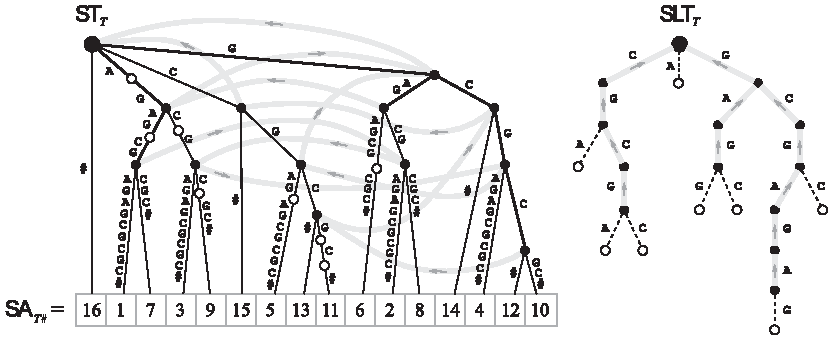
\includegraphics[width=\linewidth]{suffix-tree/st-slt-example.pdf}
    \caption{A suffix tree and its corresponding suffix link tree for $T = \texttt{AGAGCGAGAGCGCGC}$. }
\end{figure}

Moreover, the suffix links induce a subtree called the \textit{\textbf{suffix link tree}}. More formally, given a text $T$ represented by a suffix tree $(V,E)$ with suffix links, let $\ell(v)$ denote the label on the path from the root to $v$. Then, $L = \{(v,a) \mid v \in V, s(v) \in V, \ell(v) = x \ell(s(v)), x \in \Sigma\}$ be the set of all suffix links, and we define the tree $\text{SLT}(T) = (V,L)$ labeled by $\ell$ as the \textit{\textbf{suffix link tree}}.

\subsection{Count and Skip}

After reaching $s(v)$ via a suffix link, we still need to travel down the path labeled $\gamma$ in order to add a new character at the end of $\gamma$, either by branching off or creating a new leaf node. However, this walk along the $\gamma$ path takes $O(|\gamma|)$ if implemented directly. An alternative to this would be to \textit{\textbf{store the number of characters of on each edge}} and skip nodes wheneve we can.

Let $g$ denote the length of $\gamma$, the next suffix to which we want to append the new character. We start the search for the insertion point starting from $s(v)$.

\begin{marginfigure}
    \centering
    \includegraphics[width=0.8\linewidth]{suffix-tree/ukkonen-count-skip.pdf}
    \caption{\\Top: Case 1 where $g \geq g'$, skip to the next node; \\ Bottom: Case 2 where $g < g'$, go the the $g$-th character on the current edge.}
\end{marginfigure}

Recall that no two edges coming out of $s(v)$ can have labels starting with the same character. We can then use one comparison to determine the edge that we need to follow. In particular, let $h=1$ initially and before each iteration, compare the $h$th character of $\gamma$ with the first character of every edge coming out of the current node. Let $g'$ be the number of characters on the edge that we have just identified. Then, consider the following two cases:

\begin{enumerate}
    \item $g \geq g'$: Skip to the node at the end of the edge. Set $g = g - g'$, $h = h + g'$, and repeat.
    \item $g < g'$: Skip to the $g$th character on the edge and stop.
\end{enumerate}

\subsection{Edge Label Compression}

Another issue with our high-level ``algorithm'' for Ukkonen's algorithm is that every edge is explicitly labeled with the suffix they represent. A label of an edge can be as large as $\Theta(m)$, and there can be at most $\Theta(m)$ edges, making the total space required for a suffix tree $\Theta(m^2)$ in this case. This makes it impossible to build such a tree in $O(m)$ time. Fortunately, this issue can be solved using a simple trick: instead of storing the strings explicitly, we can store a pair of indicies representing the \textit{\textbf{starting and ending position of the substring}} represented by each edge. That way, each edge can be maintained using only $\Theta(\log m)$ space.

\index{word RAM model}
In the \textit{\textbf{word RAM model}}\footnote{In complexity theory, we have focused on Turing machine as our preferred model of computation. However, in analysis of algorithms, we usually use the word RAM model (often without explicitly stating it) as it is a more realistic model of how modern computers work.}, we assume that every word of size $\log m$ bits can be read and written efficiently in constant time. Hence, it is more plausible to build a suffix tree with compressed edge labels in linear time.

\subsection{Key Observations}

\newthought{No More Insertions After Type 3}

In any given phase $i+1$, if there is a Type 3 extension $j$ (the new suffix $S[j\ldots i+1]$ is already in the tree), then any further extensions in the current phase will also be of Type 3. When there is a Type 3 extension, the path labeled $S[j\ldots i]$ in the current tree must have already contained $S[i+1]$. Then clearly, so does $S[j'\ldots i]$ for all $j < j' \leq i+1$ because they are all suffixes of $S[j\ldots i]$.

\newthought{Once a Leaf, Always a Leaf}

At some point in the algorithm, if a leaf $j$ is created for the suffix starting at position $j$, then the leaf will remain a leaf throughout the algorithm. This is because the algorithm never extends a leaf. If a path leads to a leaf, it will be a Type 1 insertion, in which case we extend the edge label without explicitly adding new nodes.

\part{Dynamic Programming}

\chapter{Edit Distance}

\part{Compression and Indexing}

\chapter{Entropy and Information}

\chapter{k-mer Index and Suffix Array}
\section{Idea Behind Indexing}

Suppose you have a textbook and you want to look for a certain term, say, the word ``\textit{string}''. It would be really time-consuming, and in some cases, impossible to look for the term by going through the book page by page. That's why most books usually (and hopefully) have an index at the end, which list the pages where each term occurs.

\begin{figure}
    \centering
    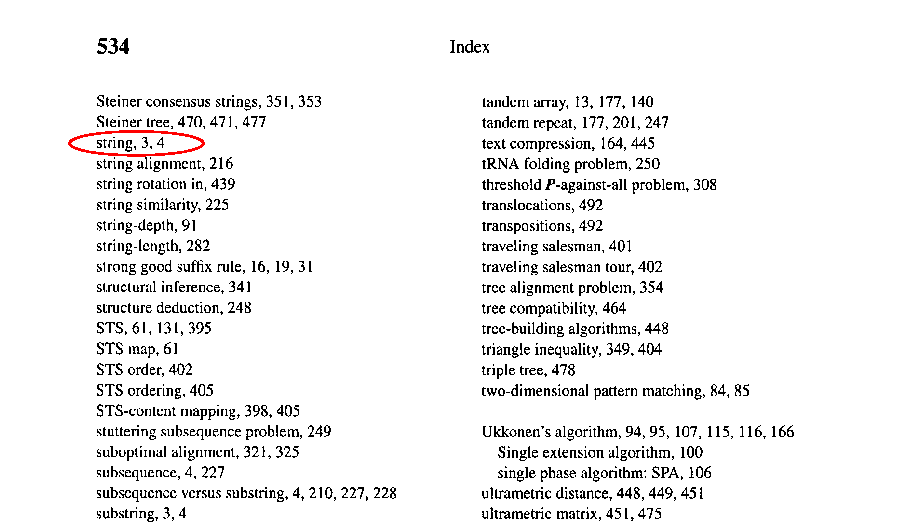
\includegraphics[width=\linewidth]{index/example-gusfield-idx.pdf}
    \label{fig:example-gusfield-idx}
    \caption{The index of Gusfield's textbook, with the term ``string'' circled.}
\end{figure}

Index can help us speed up query speed and also give us a compact representation of the data.

Two big ideas behind indexing are \textit{\textbf{grouping}} and \textit{\textbf{ordering}}. The first index that we will look at, $k$-mer index, uses grouping.

\section{\textit{k}-mer Index}

Given a text $T$, we call all its substrings of length $k$, the \textit{\textbf{k-mers}} of $T$. For example, consider the string \texttt{CGTGCGTGCTT}, it has the following 5-mers: \texttt{CGTGC}, \texttt{GCGTG}, \texttt{GTGCC}, \texttt{GTGCT}, \texttt{TGCCT}, and \texttt{TGCTT}. The substrings \textit{can have overlaps}.

$k$-mer index groups the indices of $T$ by the $k$-mer that starts at the index. So, for the string \texttt{CGTGCGTGCTT}, we have the $k$-mer index for $k=5$:

\begin{table}
    \centering
    \begin{tabular}[H]{c|c}
        $k$-mer & indices \\
        \hline
        \texttt{CGTGC} & 0, 4 \\
        \texttt{GCGTG} & 3 \\
        \texttt{GTGCC} & 1 \\
        \texttt{GTGCT} & 5 \\
        \texttt{TGCCT} & 2 \\
        \texttt{TGCTT} & 6
    \end{tabular}
\end{table}

It is easy to construct a $k$-mer index. We can scan the string from left to right and record the position of each $k$-mer. It takes $|T|-k+1$ time.

\section{Querying k-mer Index}

To query a $k$-mer index efficiently, we should first \textit{sort the index lexicographically} by the $k$-mers. It takes $k(|T|-k)\log(|T|-k) \in O(|T|^2 \log|T|)$ steps. To compare two $k$-mers, we need $k$ steps (unlike comparing two numbers or characters, which takes constant time), and sorting the list of $|T|-k$ $k$-mers takes $\Theta((|T|-k)\log(|T|-k))$. There is a bit of tradeoff here. If we choose a small $k$, we spend less time comparing two substrings during sorting, but we can possibly end with many $k$-mers in the list; in we choose a large $k$, it takes more time to compare two substrings, but we will have fewer $k$-mers to sort.

Once we sort the $k$-mer index, we can use \textit{binary search} for patterns $P$ such that $|P| \leq k$. It takes $O(|P|\log |T|)$ to query a sorted $k$-mer index. However, if $|P| > k$, $k$-mer index can be inefficient since we need to \textit{manually extend the match} once the first $k$ characters of $P$ matches a substring in $T$.

\chapter{Constructing Suffix Array}
\section{Naive Construction From Suffix Tree}

Recall that a suffix array contains the index of all suffixes of a string, sorted in lexicographic order. Hence, given a suffix tree, a suffix array can be trivially constructed through a lexicographic depth first search (that is, at each internal node, decide which path to recurse on based on the alphabetical order of the first character of each path label).

As we have seen, a suffix tree can be constructed in $O(n)$ time. It follows that a suffix array can also be constructed in $O(n)$ time using this method. However, a major issue with this approach is that we must build an intermediate suffix tree, which may require significantly more memory, and this defeats the purpose of having a suffix array in the first place, which is to have a more compact representation of the suffixes of a string.

\section{A Divide-and-Conquer Approach}

The next natural approach one might consider when presented with a problem like constructing a suffix array is divide and conquer. We are all familiar with merge sort, which runs in $O(n \log n)$ time. Constructing a suffix array similarly involves sorting the suffixes.

Let $T$ be the text for which we want to construct a suffix array. Consider the following divide-and-conquer approach:

\begin{enumerate}
    \item Divide the suffix positions into $A \subset [0\ldots n]$ and $\overline{A} = [0\ldots n] \setminus A$
    \item Construct a suffix array for $T_A$ (suffixes that start at positions in $A$) recursively
    \item Construct a suffix array for $T_{\overline{A}}$ based on the suffix array for $T_A$
    \item Merge the two suffix arrays
\end{enumerate}

The most straightforward way to divide is to divide the positions by parity (even/odd). This gives an algorithm whose runtime is given by the recurrence $T(n) = T(\lceil n/2 \rceil) + T_{merge}(n)$.

\newthought{What Goes Wrong?} Everything seems good so far, but there are two important problems: (1) how do we construct the second suffix array non-recursively, and (2) how to merge in linear time?

For a long time, finding a way to merge two suffix arrays in linear time remained an open question. The most obvious way to merge takes $O(n^2)$ time. Researchers came up with clever tricks but still only got an $O(n \log n)$ time bound. Because of that, until the early 2000s, the best known algorithm for constructing a suffix array only ran in $O(n \log n)$ time.

In 2003, Karkkainen and Sanders published their seminal paper (along with some other researchers who independently published similar results around the same time), which proposed one of the first linear time algorithms for constructing a suffix array. It uses the same divide-and-conquer framework, with a little twist.

\section{Karkkainen-Sanders Algorithm}

Karkkainen and Sanders' algorithm uses the same divide-and-conquer approach, but instead of dividing the positions into even and odd positions like previous researchers have done, they divided the positions $i$'s into those with $i \bmod 3 \neq 0$ and $i \bmod 3 = 0$. This, along with a neat trick during merging, is enough to give us an $O(n)$ time algorithm for construct a suffix array.

Let's first recall the general framework for constructing suffix array using divide-and-conquer

\begin{codebox}
    \Procname{$\proc{Karkkainen-Sanders}$}
    \li construct suffix array for suffixes starting at positions $i \bmod 3 \neq 0$ \\recursively \Comment{$T(2/3 n)$ }
    \li construct suffix array for suffixes starting at positions $i \bmod 3 = 0$ \\ using results from step 1 \Comment{$O(n)$}
    \li merge the two suffix arrays \Comment{$O(n)$}
\end{codebox}

We will see how to perform each step within the given time. We call the suffixes starting at positions $i \bmod 3 \neq 0$ the \textit{\textbf{sample suffixes}}, and the suffixes starting at positions $i \bmod 3 = 0$ the \textit{\textbf{non-sample suffixes}}.

\subsection{Sorting The Sample Suffixes, Recursively}

Given a string $T$ of length $n$, we define $T[j]$ for all $j > n$ to be equal to \texttt{\$}, so $T[j] = \texttt{\$}$ for all positions beyond $n$. This is just to avoid having to deal with the edge cases.

Let $t_0$ be the set of \textbf{triples} (not suffixes) starting at position $i \bmod 3 = 0$, so $t_0 = \{ T[i\ldots i+2] \mid i \bmod 3 = 0, \, i \leq n \}$. Similarly, let $t_1$ and $t_2$ be the sets of triples starting at position $i \bmod 3 = 1$ and 2, respectively. For example, suppose $T = \texttt{dadbcddadbcd\$}$ with the delimiter $\$$ in the end, we will have
$$
t_1 = \{\texttt{dad},\,\texttt{bcd},\,\texttt{dad},\,\texttt{bcd},\,\texttt{\$\$\$}\}
$$
and
$$
t_2 = \{ \texttt{adb},\, \texttt{cdd},\, \texttt{adb},\, \texttt{cd\$} \}
$$
To sort the suffixes starting at positions $i \bmod 3 \neq 0$, we first sort the triples in $t_1 \cup t_2$. This can be done in $\Theta(n)$ time using \textbf{radix sort}. For $x \in t_1 \cup t_2$, we define the \textbf{rank} $\id{rank}(x)$ to be the order of the triple $x$ in the sorted list of $t_1 \cup t_2$. If two triples have the same order in the sorted list, they will have the same rank. Further, for a set of triples $X$, we define $\id{Rank}(X)$ to be the list of ranks for each triple in the sorted order. That is, the $i$th element of $\id{Rank}(X)$ will be $\id{rank}(X[i])$. Using the same example as above where $T = \texttt{dadbcddadbcd\$}$, we have
$$
\begin{array}{ccccccccccc}
    \id{pos} & = & 13 & 2 & 8 & 4 & 10 & 11 & 5 & 1 & 7 \\
    \id{Sorted}(t_{1,2}) & = & \texttt{\$\$\$} & \texttt{adb} & \texttt{adb} & \texttt{bcd} & \texttt{bcd} & \texttt{cd\$} & \texttt{cdd} & \texttt{dad} & \texttt{dad} \\
    \id{Rank}(t_{1,2}) & = & 1 & 2 & 2 & 3 & 3 & 4 & 5 & 6 & 6
\end{array}
$$
We also record $\id{pos}$, the starting position of each of the triple in the original string.

Now, let us go back to the original set of triples, $t_1$ and $t_2$. We create a new string $t'$ equals to $t_1 \cdot t_2$ ($t_1$ concatenated with $t_2$) with each triple \textbf{mapped to its rank}.

$$
\begin{array}{ccccccc|cccc}
    \id{pos} & = & 1 & 4 & 7 & 10 & 13 &  2 & 5 & 8 & 11 \\
    t_1 \cdot t_2 & = & \texttt{dad} & \texttt{bcd} & \texttt{dad} & \texttt{bcd} & \texttt{\$\$\$} & \texttt{adb} & \texttt{cdd} & \texttt{adb} & \texttt{cd\$} \\
    t' & = & 6 & 3 & 6 & 3 & 1 & 2 & 5 & 2 & 4
\end{array}
$$

Next, we \textbf{recursively find the suffix array} for $t'$. We claim that the suffix array for $t'$ specifies the suffix array for $S$ restricted to the suffixes starting at positions $i \bmod 3 \neq 0$.

\newthought{Wait! But Why?}

\textit{Claim}. Suffix array for $t'$ specifies the suffix array for $S$ restricted to the suffixes starting at positions $i \bmod 3 \neq 0$

To see why this is true, we first prove this lemma.

\begin{lemma}
    Let $t_i'$ and $t_j'$ be two suffixes of $t'$ starting at position $i$ and $j$, respectively. If $s_i' \prec_{lex} s_j'$ (if $s_i'$ is lexicographically less than $s_j'$), then the suffix of the original string $T$ starting at position $\id{pos}[i]$ is also lexicographically smaller than the suffix of $T$ starting at position $\id{pos}[j]$.
\end{lemma}

\begin{proof}
    Recall that $t'$ can be divided into two parts. The first half contains the ranks of triples whose first character starts at position $i \bmod 3 = 1$. The second half contains the ranks of triples whose first character starts at position $i \bmod 3 = 2$. To prove the lemma, we consider the following cases regarding the positions of $i$ and $j$ in $t'$.

    \textbf{Case 1}: Both $i$ and $j$ are in the first half. Then, $\id{pos}[i] = \id{pos}[j] = 1 \mod 3$. We first observe that the comparison of the two suffixes starting at $i$ and $j$ \textbf{will not go beyond the boundary} between the first and the second half.
    \begin{marginfigure}
        \includegraphics[width=\linewidth]{sa-dc3/case1-t-prime-suffixes.pdf}
    \end{marginfigure}
    More formally, let $k$ be the position such that $\id{pos}[k] \bmod 3 = 1$ but $\id{pos}[k+1] \bmod 3 = 2$. Then, during the comparison of the two suffixes of $t'$ starting at $i$ and $j$, at most $k$ characters are compared. This is because the triple at position $\id{pos}[k]$ will contain the unique \textbf{null terminator} that is lexicographically smaller than any character in the alphabet, thus giving the triple at $\id{pos}[k]$ a \textbf{unique rank}.

    Moreover, each symbol in $t'$ represents the \textbf{rank of a triple} starting at that position in $T$. By assumption, the suffix of $t'$ starting at $i$ is lexicographically smaller than the suffix of $t'$ starting at $j$. Then, there must exists some $c$ such that $t'[i+c] < t'[j+c]$. This implies that the triple starting at position $\id{pos}[j+c]$ that is lexicographically larger than the triple starting at position $\id{pos}[i+c]$ because $t'$ represents the ranks of the triples. The presence of this \textbf{lexicographically larger triple} makes the suffix of the original string at $\id{pos}[i]$ lexicographically smaller than the suffix at $\id{pos}[j]$.
    
    \textbf{Case 2}: Both $i$ and $j$ are in the second half. This case follows from a similar argument as Case 1.

    \begin{marginfigure}
        \includegraphics[width=\linewidth]{sa-dc3/case3-t-prime-suffixes.pdf}
    \end{marginfigure}

    \textbf{Case 3}: $i$ is in the first half and $j$ is in the second half. As in the first two cases, the comparison will \textbf{never cross the boundary}. This, again, is due to the distinct null terminator symbol. In particular, the triple starting at $\id{pos}[k]$ (recall that $k$ is the boundary between the two parts) contains at least one more/fewer null terminator symbol compared to the triple at $\id{pos}[|t'|]$. Hence, the triple at $\id{pos}[k]$ will have a \textbf{unique rank}, which helps us \textbf{break the tie} after the comparison at position $k$. We can always determine the lexicographic order of the two suffixes without crossing the boundary.

    Now, going back to $t'$, if we have the suffix of $t'$ starting at $i$ being lexicographically smaller than the suffix of $t'$ starting at $j$, we know that there must be some $c$ such that $t'[i+c] < t'[j+c]$, which implies the rank of some triple at $\id{pos}[i+c]$ is lexicographically smaller than that at $\id{pos}[j+c]$. Since we never cross the boundary when comparing the suffixes of $t'$ starting at $i$ and $j$, we are always comparing the rank of a contiguous and non-overlapping substring of $T$ starting at $\id{pos}[i]$ with the rank of some other contiguous and non-overlapping substring of $T$ at $\id{pos}[j]$ without ever going backward in the comparison (because we don't cross the boundary). Then, it follows that the lexicographic ordering of the ranks in $t'$ implies the ordering in $T$.
    
    \textbf{Case 4}: $i$ is in the second half and $j$ is in the first half. This follows from a similar argument as Case 3.

    In all cases, the implication holds, so the lemma holds.
\end{proof}

One important takeaway from the proof of this lemma is that the null terminator symbol \texttt{\$} is a tie-breaker, giving us unique ranks for triples at the end of the first and second half so that we never cross the boundary between the two halves. This unique rank, in turn, allows us to use the string of ranks to implicitly sort the suffixes in the original string $T$.

Using our previous example with
$$
\begin{array}{ccccccc|cccc}
    \scriptstyle i &  & \scriptstyle 1 & \scriptstyle 2 & \scriptstyle 3 & \scriptstyle 4 & \scriptstyle 5 & \scriptstyle 6 & \scriptstyle 7 & \scriptstyle 8 & \scriptstyle 9 \\
    \id{pos} & = & 1 & 4 & 7 & 10 & 13 &  2 & 5 & 8 & 11 \\
    t_1 \cdot t_2 & = & \texttt{dad} & \texttt{bcd} & \texttt{dad} & \texttt{bcd} & \texttt{\$\$\$} & \texttt{adb} & \texttt{cdd} & \texttt{adb} & \texttt{cd\$} \\
    t' & = & 6 & 3 & 6 & 3 & 1 & 2 & 5 & 2 & 4
\end{array}
$$
we have
$$
\begin{array}{ccccccccccc}
    \text{SA for $t'$} & = & 5 & 8 & 6 & 4 & 2 &  9 & 7 & 3 & 1 \\
    \text{SA$_{12}$ for $T$} & = & 13 & 8 & 2 & 10 & 4 & 11 & 5 & 7 & 1
\end{array}
$$
The $i$th entry in the SA for $T$ is $SA_{12}(T)[i] = \id{pos}[SA(T')[i]]$. Here, $SA_{12}(T)$ refers to the suffix array for the original string $T$ but only considering the suffixes at positions $1$ or $2$ mod $3$.

\subsection{Sorting the Non-Sample Suffixes}

There is an easy way to sort the non-sample suffixes. Those are the suffixes that start at positions $i \bmod 3 = 0$. Again, we begin by considering the triples starting at these positions. Each of such positions is followed by two positions with $i \bmod 3 \neq 0$. Ordering of the triples starting at one and two positions after those with $i \bmod 3 = 0$ have already been determined recursively as discussed in the previous subsection. We can then use the information we know about the sample suffixes to sort the non-sample suffixes in linear time, non-recursively.

To this end, we construct a list $t''$ that contains all characters at positions $i \bmod 3 = 0$ with each character followed by the rank of the suffixes starting at position immediately after $i$ (which can be determined from $SA[t']$ that we have constructed in the previous step).

Slightly more formally, the $i$th element of $t''$ will be
$$
t''[i] = T[3i] \cdot SA_{12}(T)[3i+1]
$$
In our example, $T = \texttt{dadbcddadbcd\$}$ and
$$
\begin{array}{ccccccccccc}
    \scriptstyle i &  & \scriptstyle 1 & \scriptstyle 2 & \scriptstyle 3 & \scriptstyle 4 & \scriptstyle 5 & \scriptstyle 6 & \scriptstyle 7 & \scriptstyle 8 & \scriptstyle 9 \\
    \text{SA for $t'$} & = & 5 & 8 & 6 & 4 & 2 &  9 & 7 & 3 & 1 \\
    \text{SA$_{12}$ for $T$} & = & 13 & 8 & 2 & 10 & 4 & 11 & 5 & 7 & 1
\end{array}
$$
so
$$
\begin{array}{ccccccccccc}
    \text{triple} & = & \texttt{dbc} & \texttt{dda} & \texttt{dbc} & \texttt{d\$\$} \\
    t'' & = & \texttt{d5} & \texttt{d8} & \texttt{d4} & \texttt{d1} \\
    \id{pos} & = & 3 & 6 & 9 & 12
\end{array}
$$
We sort $t''$ using radix sort in $\Theta(n)$ time. For our example, this gives us
$$
\begin{array}{ccccccccccc}
    t'' & = & \texttt{d1} & \texttt{d4} & \texttt{d5} & \texttt{d8} \\
    \id{pos} & = & 12 & 9 & 3 & 6
\end{array}
$$
The corresponding positions in the sorted $t''$ is the suffix array for the suffixes starting at $i \bmod 3 = 0$, so we have $SA_{3}(T)$ as well.

The correctness of this step is trivial from the correctness of radix sort and the fact that the entries in $SA_{12}$ are unique (so there won't be tie).

\subsection{Merging the Two Suffix Arrays}

The final punchline. We will merge $SA_{12}(T)$ and $SA_{3}(T)$ into one suffix array in linear time.

Recall that in the $O(n^2)$ algorithm for constructing a suffix array, the merging is done in $O(n^2)$ time using the naive method. The naive method keeps two pointers to each of the restricted suffix arrays $SA_{12}$ and $SA_{3}$. It then compare the suffixes explicitly in worst-case $O(n)$ time. We do this for all the $O(n)$ pairs of positions, giving us an $O(n^2)$ time algorithm.

\begin{codebox}
    \li $i,j = 1,1$ 
    \li \While $i \leq |SA_{12}(T)|$ and $j \leq |SA_{3}(T)|$  \Do
            \li compare suffixes $T[SA_{12}(T)[i] \ldots]$ and $T[SA_{12}(T)[j] \ldots]$
            \li update $i,j$ accordingly
\end{codebox}

However, with the suffixes arrays $SA_{12}$ and $SA_3$, we can actually do the comparison in constant time. For each arbitrary pair of positions $i,j$, we only need at most $3$ explicit character comparisons before we reach a position $i',j'$ such that $i' = j' \mod 3$, at which point the lexicographic order of the two suffixes can be determined using an $O(1)$ \textbf{lookup} in the appropriate restricted suffix array.

For a more detailed procedure for merging, consider the following cases:

\textbf{Case 1}: Compare two suffixes starting at $i$ and $j$ where $i \bmod 3 = 2$ and $j \bmod 3 = 0$. If the encounter a character such that $T[i] \neq T[j]$, then we are done. Otherwise, continue comparing $T[i]$ with $T[j]$ and updating $i$ and $j$. After at most 2 comparisons, $i \bmod 3 = 1$ and $j \bmod 3 = 2$. We can determine the ordering of the two suffixes by comparing the locations of $i$ and $j$ in $SA_{12}$ in $O(1)$ time.

\textbf{Case 2}: Compare two suffixes starting at $i$ and $j$ where $i \bmod 3 = 1$ and $j \bmod 3 = 0$. If we encounter a character such that $T[i] \neq T[j]$, then we are done. Otherwise, the problem reduces to Case 1, and we can determine the lexicographic ordering of the suffixes starting at $i$ and $j$ with at most $3$ explicit comparisons.

\textbf{Case 3}: $i = j \mod 3$. This case is trivial through a constant-time lookup in $SA_{12}$ if $i \bmod 3 = j \bmod 3 \neq 0$ or in $SA_{3}$ if $i \bmod 3 = j \bmod 3 = 0$.

In all three cases, we can determine the lexicographic ordering of the two suffixes within $O(1)$ comparisons. We repeat this for all $|T|$ positions, giving us an $O(n)$ time algorithm for merging.

\subsection{Wrapping It Up}

And here we have it, the linear-time algorithm for constructing a suffix array. At first glance, it appears to be quite a sophisticated algorithm, but the ideas behind it are actually quite fundamental. It based on the same divide-and-conquer approach that previous $O(n^2)$ and $O(n \log n)$ time algorithms have used, but with a few ingenious improvements that allow us to do the merging in $O(n)$ time. Note that the linear-time merging is not possible if we divide the suffixes up into positions $0$ or $1$ mod $2$ since we are not guaranteed to be at a position $i=j \mod 2$ after just a constant number of comparisons.

As we mentioned at the beginning, this algorithm is due to Karkkainen and Sanders. It is often referred to as the \textit{\textbf{Karkkainen-Sanders (KS) algorithm}} or the \textit{\textbf{DC3 algorithm}} since it is a divide-and-conquer algorithm that divides the positions based on their values modulo 3.

To wrap this section up, let us prove that the KS algorithm indeed runs in linear time.

\begin{theorem}
    The suffix array for text $T$ of length $n$ can be computed in time $O(n)$.
\end{theorem}

\begin{proof}
    We use the Karkkainen-Sanders' algorithm. The correctness of the algorithm is argued as we introduce the algorithm. Now, we consider the runtime of the algorithm.

    Sorting of the triples takes $O(n)$ time using radix sort, and so does the computation of the SA for the non-sample suffixes at position $i \bmod 3 = 0$. At each level of the recursion, the suffix array that we recursively construct is of size $\lceil 2/3n \rceil$. Finally, merging takes $O(n)$ time. Hence, the overall runtime is given by the recurrence
    $$
    \begin{aligned}
        T(n) &= T(\lceil 2/3n \rceil) + 3O(n) \\
        &= T(\lceil 2/3n \rceil) + O(n) \\
        &\leq n \sum_{i=0}^\infty \left( \frac{2}{3} \right)^i \\
        &\in O(n) 
    \end{aligned}
    $$
    The same recurrence can also be solved using the Master's theorem.
\end{proof}

\chapter{Burrows-Wheeler Transform}

\chapter{FM Index}

\chapter{Wavelet Tree}

\backmatter

\bibliographystyle{abbrvnat}
\bibliography{stringbook}
\addcontentsline{toc}{chapter}{Bibliography}

\printindex

\end{document}

